
\chapter{Systembeskrivelse}
Universal Actuator Drive består af to overordnede blokke - et power-modul, der står for effektkonverteringen i converteren, og et PWM-modul der sikrer reguleringen af converterens udgang. Power-modulet består af en transformator og en MOSFET til convertering af udgangsbelastningen, samt et indgangs- og et udgangsfilter for filtrering af højfrekvent støj.

PWM-modulet består af to reguleringssløjfer, der regulerer udgangen efter både udgangsstrømmen og -spændingen. Denne regulering sker ved at regulere duty-cyclen af det PWM-signal der driver MOSFET'en. Disse funktionaliteter er inkluderet i én PWM-controller. 

På figur~\ref{fig:flowdiagram} ses et flowdiagram over konceptet af Universal Actuator Drive. Det giver et overblik over hvilke scenarier, og eksterne valg, der kan påvirke flowet i systemet. Her det især valg af udgangsbelastning, og de to reguleringssløjfer der påvirker systemets udgang. 

\begin{figure}[H]
	\centering
	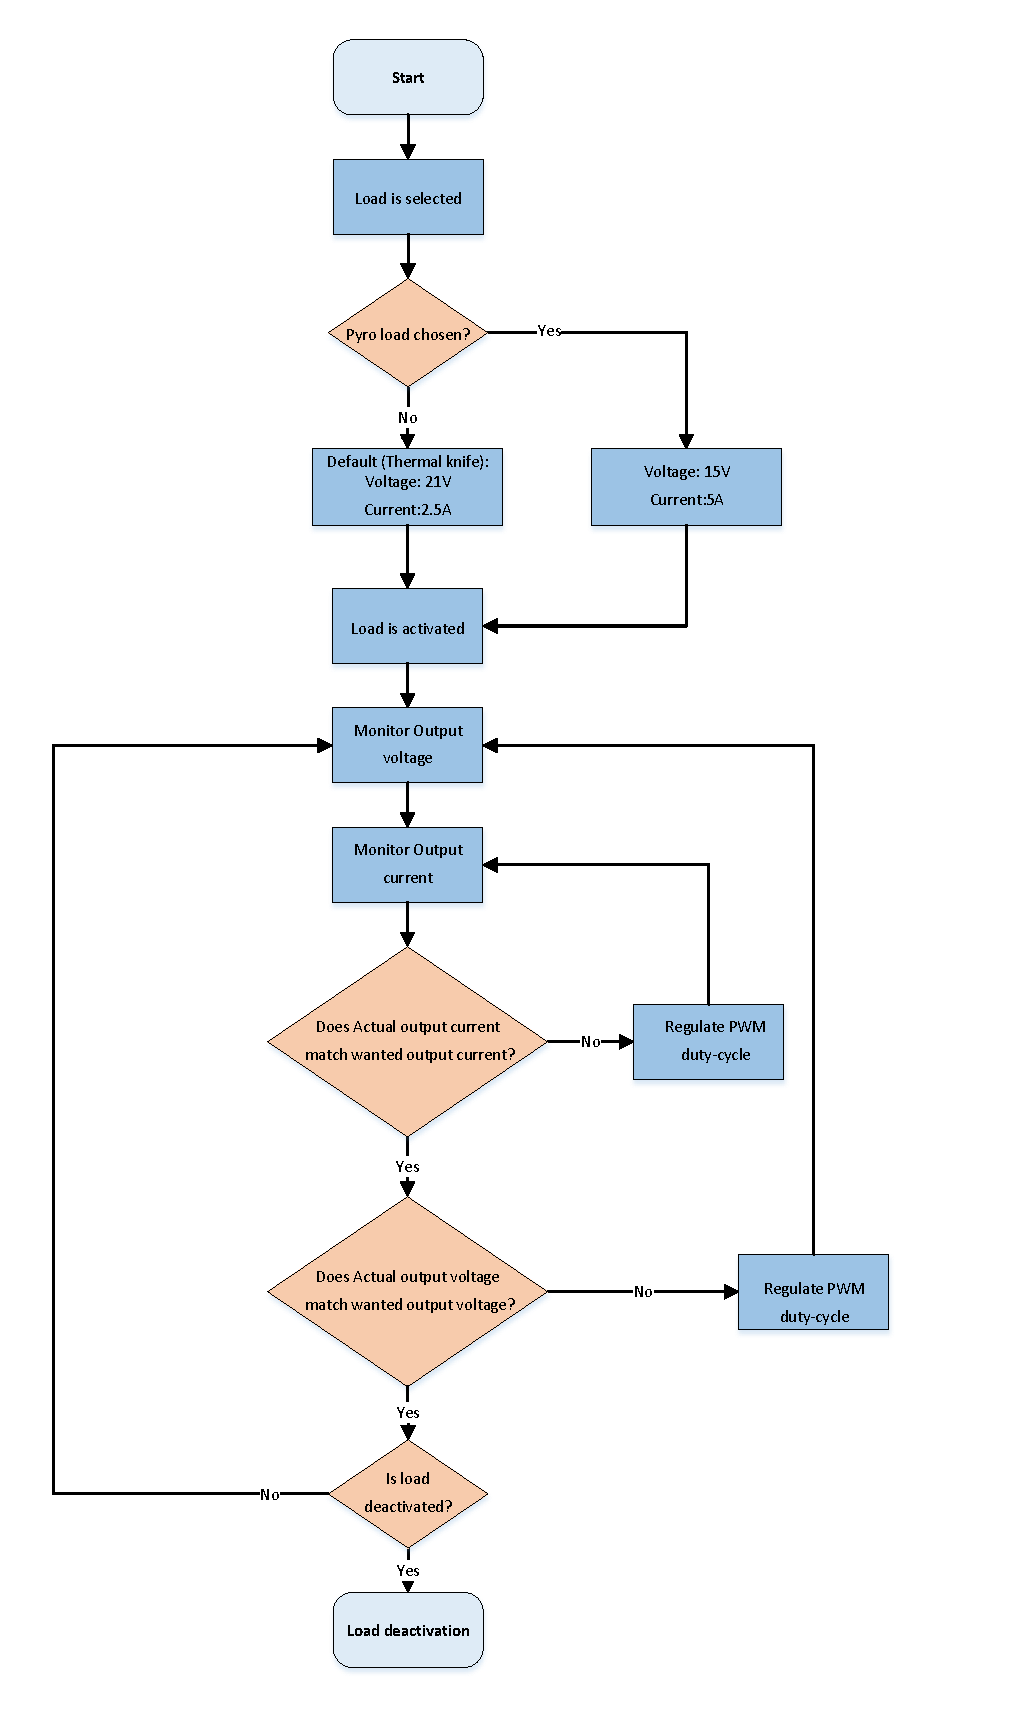
\includegraphics[width=0.7\linewidth]{../Dokumentation/tex/kravspecifikation/billeder/Flow_diagram.pdf}
	\caption{Flowdiagram for Universal Actuator Drive}
	\label{fig:flowdiagram}
\end{figure}